\documentclass{ximera}

\title{Oefeningen op differentiële analysemethode}
\author{Mila Vervoort}
\license{CC: 0}         % replace with an appropriate license, or set it in xmPreamble

\begin{document}
\begin{abstract}
    Oefeningen op integrale analysemethode voor batch experimenten.
\end{abstract}
\maketitle
\label{xim:oefeningen differentiële analysemethode}

\section*{Oefening 1: $n^{de}$ orde reactie}

Dit is dezelfde oefening als bij de integrale analysemethode. We gaan deze nu proberen op te lossen met de differentiële analysemethode.

\textbf{Gegeven}

De gasfase ontbinding van di-\textit{tert}-butylperoxide in producten ethaan en aceton gebeurt volgens de reactie:

\[
(\mathrm{CH}_3)_3\mathrm{COOC}(\mathrm{CH}_3)_3 \rightarrow \mathrm{C}_2\mathrm{H}_6 + 2\,\mathrm{CH}_3\mathrm{COCH}_3
\]
of symbolisch:
\[
A \rightarrow R + 2S
\]

Er werden experimenten uitgevoerd in een isotherme batchreactor. De totale druk werd gemeten als functie van de tijd:

\begin{center}
\begin{tabular}{c|c}
$t$ (min) & $p$ (mmHg) \\
\hline
0.0 & 7.5 \\
5.0 & 12.5 \\
10.0 & 15.8 \\
15.0 & 17.9 \\
20.0 & 19.4 \\
\end{tabular}
\end{center}

\textbf{Gevraagd}

Gebruik de differentiële analysemethode om te bepalen welke orde deze reactie heeft en wat de reactieconstante is. \\

\begin{remark} \text{  }

Met behulp van de differentiële analysemethode kunnen zowel de reactieorde $n$ als de reactieconstante $k$ gelijktijdig uit de experimentele gegevens worden bepaald. Dit vormt een belangrijk voordeel ten opzichte van de integrale analysemethode, waarbij vooraf een reactieorde moet worden verondersteld.
\end{remark}

\begin{question} \textbf{Linearisatie van de reactiekinetiek}
\\
De snelheidsvergelijking voor een nde orde reactie is 
\[
\frac{dC_A}{dt} = -kC_A ^n
\]
Uit de vorige oefening weten we al dat het verband tussen concentratie $C_A$ en de druk $p$ gegeven wordt door volgende vergelijking:
    \[
    C_A = \frac{3p_0-p}{2RT}
    \]
Deze uitdrukking invullen geeft: 
\[
\frac{-1}{2RT}\frac{dp}{dt} = -k(\frac{3p_0-p}{2RT})^n
\]
\[
\frac{dp}{dt} = k(\frac{1}{2RT})^{n-1}(3p_0-p)^n
\]
Vervang $k$ door $k' = k(\frac{1}{2RT})^{n-1}$
\[
\frac{dp}{dt} = k'(3p_0-p)^n
\]
Herschrijf deze vergelijking zodanig dat zowel $k'$ als $n$ gelijktijdig kunnen worden bepaald. De meest geschikte vorm is:

    \begin{multipleChoice}
            \choice{$\ln(\frac{dp}{dt})= \ln(k')+\ln(3p_0-p)^n$}
            \choice{$\ln(\frac{dp}{dt})= n\ln(k'(3p_0-p))$}
            \choice[correct]{$\ln(\frac{dp}{dt})= \ln(k')+n\ln(3p_0-p))$}
    \end{multipleChoice}
    \begin{feedback} \text{  }
    
        Als de snelheidsvergelijking in deze vorm geschreven wordt, kunnen $n$ en $k'$ eenvoudig bepaald worden.
        \[
        \underbrace{\ln \left(\frac{dp}{dt}\right)}_{y}
        =
        \underbrace{\ln k'}_{\text{intercept}}
        +
        \underbrace{n}_{\text{helling}}
        \,
        \underbrace{\ln(3p_0 - p)}_{x}
        \]
    \end{feedback}

\end{question}

\begin{remark} \textbf{Bepalen van de reactiesnelheid met centrale differentie}

De experimentele gegevens bestaan uit discrete metingen van de druk als
functie van de tijd. Om de reactiesnelheid te bepalen, moet de afgeleide
$\frac{dp}{dt}$ berekend worden.

Omdat de druk enkel op discrete tijdstippen gekend is, wordt de afgeleide
benaderd met een centrale differentiebenadering. Hierbij wordt de helling
tussen twee opeenvolgende meetpunten gebruikt als een schatting van de
afgeleide in het tussenliggende tijdstip:

\[
f'\left(t_{n+\frac{1}{2}}\right)
\approx
\frac{f(t_{n+1})-f(t_n)}
{t_{n+1}-t_n}
\]

Er ontstaan hierdoor nieuwe intermediaire tijdstippen tussen de oorspronkelijke metingen. Op deze tijdstippen wordt de reactiesnelheid bepaald als:

\[
\left(\frac{dp}{dt}\right)_{n+\frac{1}{2}}
\approx
\frac{p_{n+1}-p_n}{t_{n+1}-t_n}
\]

Deze berekende snelheden worden vervolgens gebruikt in de gelineariseerde kinetische vergelijking.
\end{remark}


\begin{question} \textbf{Bepalen van de reactiesnelheid uit de experimentele data}\\

Gebruik de Python-code in de volgende Google Colab-file. Vul de ontbrekende regels aan om de berekeningen uit te voeren.

\begin{center}
\href{https://colab.research.google.com/drive/1dWckfscjsUmQ97Mw7P00nvdMTTST00n3?usp=sharing}{\Large Open de Google Colab notebook}
\end{center}

De code berekent voor alle meetpunten de intermediaire tijdstippen en de bijhorende waarden van $\frac{dp}{dt}$ met behulp van de differentiebenadering.

Controleer of de methode correct wordt toegepast door het eerste tijdsinterval tussen $t=0$ min en $t=5$ min handmatig te analyseren.
\begin{enumerate}
    \item Wat is het intermediaire tijdstip?
    \[
    t = \answer{2.5}\ \text{min}
    \]
    \begin{feedback}
    Het intermediaire tijdstip ligt halverwege de twee meetpunten:
    \[
    t_{n+\frac{1}{2}}=\frac{t_n+t_{n+1}}{2}
    \]
    Voor het eerste interval:
    \[
    t_{1/2}=\frac{0+5}{2}=2.5\ \text{min}
    \]
    \end{feedback}

    \item Wat is de druk op dit intermediaire tijdstip?
    \[
    p = \answer{10.0}\ \text{mmHg}
    \]
       \begin{feedback}
    De druk op het intermediaire tijdstip wordt benaderd als het gemiddelde van
    de twee omliggende meetpunten:
    \[
    p_{n+\frac{1}{2}}=\frac{p_n+p_{n+1}}{2}
    \]
    Dus:
    \[
    p_{1/2}=\frac{7.5+12.5}{2}=10.0\ \text{mmHg}
    \]
    \end{feedback}

    \item Bereken de afgeleide $\dfrac{dp}{dt}$ op dit intermediaire tijdstip met de centrale differentiebenadering.
    \[
    \frac{dp}{dt}=\answer{1.00}\ \text{mmHg/min}
    \]
    \begin{feedback}
    De reactiesnelheid wordt benaderd als de helling tussen de twee
    opeenvolgende meetpunten:
    \[
    \left(\frac{dp}{dt}\right)_{n+\frac{1}{2}}
    \approx
    \frac{p_{n+1}-p_n}{t_{n+1}-t_n}
    \]

    Voor het eerste interval:
    \[
    \frac{dp}{dt}
    =
    \frac{12.5-7.5}{5-0}
    =
    1.00\ \text{mmHg/min}
    \]
    \end{feedback}
\end{enumerate}

Dezelfde berekening kan vervolgens automatisch worden uitgevoerd voor alle
tijdintervallen in de Google Colab-file.

\iffalse
\begin{table}[h!]
\centering
\begin{tabular}{c|c||c|c|c}
$t$ [min] & $p$ [mmHg] & $t$ [min] &$p$ [mmHg] & $\frac{dp}{dt}$ \\
\hline
0.0  & 7.50  &  & & \\
     &       & 2.50   & 10   & 1.00  \\
5.0  & 12.50 &  & &    \\
     &       &   7.50     & a & 0.66\\
10.0    &   15.80    &   &    &  \\
&  & 12.50 & 16.85 & b     \\
  15.0   & 17.90       &       &  & \\
 & & 17.50 & 16.85 & 0.30   \\
20.0 & 19.40 &       &  &     \\
\end{tabular}
\end{table}

Vul de tabel  verder aan:
\[a = \answer{14.15}\]
\[b = \answer{0.42}\]
\fi 
\end{question}

\begin{question} \textbf{Data verwerken}\\

De waarden van $\frac{dp}{dt}$ zijn nu bepaald. Om de reactieorde en
reactieconstante te bepalen, worden deze waarden verwerkt volgens de
gelineariseerde kinetische vergelijking.

Bepaal in de Google Colab-file de overeenkomstige $x$- en $y$-waarden en controleer de bekomen resultaten aan de hand van onderstaande tabellen.

Welke tabel komt overeen met de resultaten die je uit de berekeningen hebt verkregen?

\begin{multipleChoice}
    \choice[correct]{\begin{tabular}{c|c}
    $\ln(3p_0 - p)$ & $\ln\!\left(\frac{dp}{dt}\right)$ \\
    \hline
    2.53 & 0.00 \\
    2.12 & -0.42 \\
    1.73 & -0.87 \\
    1.35 & -1.20 \\
    \end{tabular}} 

    \choice{\begin{tabular}{c|c}
    $\ln(3p_0 - p)$ & $\ln\!\left(\frac{dp}{dt}\right)$ \\
    \hline
    2.53 & 0.00 \\
    2.12 & -0.34 \\
    1.73 & -0.90 \\
    1.35 & -1.35 \\
    \end{tabular}} 
    
    \choice{\begin{tabular}{c|c}
    $\ln(3p_0 - p)$ & $\ln\!\left(\frac{dp}{dt}\right)$ \\
    \hline
    2.40 & 0.00 \\
    2.00 & -0.42 \\
    1.60 & -0.87 \\
    1.20 & -1.20 \\
    \end{tabular}} 
\end{multipleChoice}


\end{question}

\begin{question} \textbf{Interpreteren van de plot }\\

Maak in de Google Colab-file vervolgens een plot van de de berekende waarden en maak een lineaire fit doorheen de punten. De code is al volledig geschreven, voer deze enkel nog uit en los de volgende vraag op.

\iffalse
    De verzamelde data kan nu geplot worden in een $\ln(\frac{dp}{dt})$ versus $\ln(3p_0-p)$ plot.
\pgfplotsset{compat=1.18}
\begin{figure}[h!]
\centering
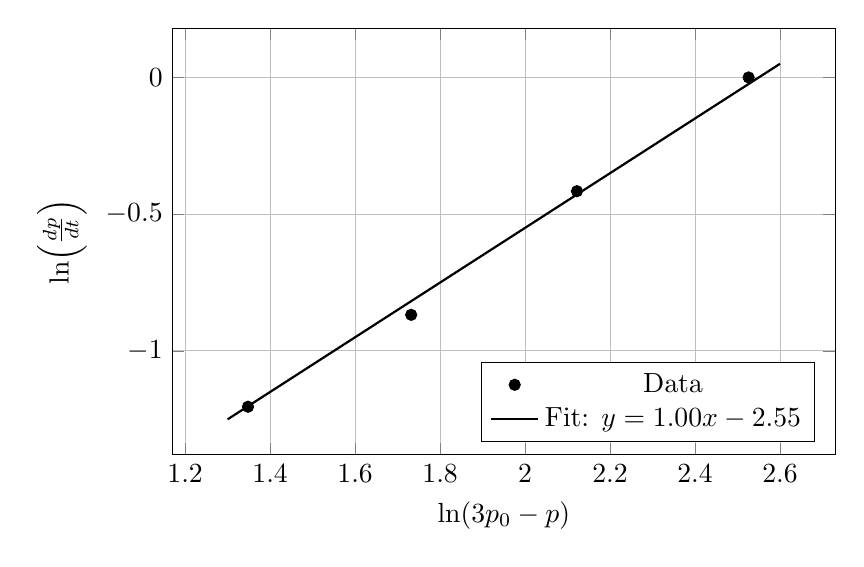
\begin{tikzpicture}
\begin{axis}[
    width=10cm,
    height=7cm,
    xlabel={$ \ln(3p_0 - p) $},
    ylabel={$ \ln\!\left(\frac{dp}{dt}\right) $},
    grid=major,
    legend pos=south east
]
% Datapunten
\addplot[
    only marks,
    mark=*,
] coordinates {
    (2.526, 0.00)
    (2.122, -0.416)
    (1.732, -0.868)
    (1.348, -1.204)
};
\addplot[
    domain=1.3:2.6,
    samples=100,
    thick
] {1.0*x - 2.55};
\legend{Data, Fit: $y = 1.00x - 2.55$}
\end{axis}
\end{tikzpicture}
\end{figure}
\fi

Welke waarde hebben $n$ en $k$ volgens deze plot?
\[n = \answer{1.04}\]
\[k = \answer{0.073}\]
\begin{feedback} .
\newline
    De helling van de rechte: $n = 1.04$. \\
    Het intercept van de rechte: $\ln(k') = -2.623$.
    \[\ln(k') = \ln(k(\frac{1}{2RT})^{n-1}) = \ln{k} = -2.623\]
    \[k = 0.073\]
\end{feedback}
\end{question}
\text{  } \\

\section*{Oefening 2: Rotte appel kinetiek}

\textbf{Gegeven}

De reactiekinetiek van de reactie wordt verondersteld als volgt:
\[
-R_A = \frac{k_1 C_A}{(1 + k_2 C_A)^2}
\]
Er worden experimentele metingen gedaan waaruit volgende data wordt gehaald:
\begin{center}
\begin{tabular}{c|c}
$t$ (h) & $C_A$ (mol/L) \\
\hline
0 & 1.00 \\
1 & 0.83 \\
2 & 0.71 \\
3 & 0.62 \\
4 & 0.55 \\
5 & 0.50 \\
\end{tabular}
\end{center}

\textbf{Gevraagd}

Bepaal de waarden van $k_1$ en $k_2$.

\begin{question} \textbf{Linearisatie van de reactiekinetiek}

Probeer de snelheidsvergelijking om te vormen naar een lineaire vorm waarbij de gezochte waarden makkelijk zouden moeten kunnen afgelezen worden van een grafiek.

Welke van de onderstaande linearisaties is correct?
\begin{multipleChoice}
\choice{$\dfrac{C_A}{-R_A} = \dfrac{1}{k_1} + \dfrac{k_2}{k_1} \sqrt{C_A}$}

\choice{$\dfrac{C_A}{-R_A} = \dfrac{1}{k_1} + \dfrac{k_2}{k_1} C_A$}

\choice[correct]{$\sqrt{\dfrac{C_A}{-R_A}} = \dfrac{1}{\sqrt{k_1}} + \dfrac{k_2}{\sqrt{k_1}} C_A$}

\choice{$\sqrt{\dfrac{C_A}{-R_A}} = \dfrac{1}{k_1} + \dfrac{\sqrt{k_2}}{k_1} C_A$}
\begin{feedback}
    \[
    - R_A = \frac{k_1 C_A}{(1 + k_2 C_A)^2}
    \]
    
    Neem het omgekeerde en vermenigvuldig met $C_A$:
    \[
    \frac{C_A}{-R_A} = \frac{(1 + k_2 C_A)^2}{k_1}
    \]
    
    Neem de wortel:
    \[
    \sqrt{\frac{C_A}{-R_A}} = \frac{1 + k_2 C_A}{\sqrt{k_1}}
    \]
    Herschrijf:
    \[
    \underbrace{\sqrt{\frac{C_A}{-R_A}}}_{y}
    =
    \underbrace{\frac{k_2}{\sqrt{k_1}}}_{\text{helling}}
    \;
    \underbrace{C_A}_{x}
    +
    \underbrace{\frac{1}{\sqrt{k_1}}}_{\text{intercept}}
    \]
\end{feedback}
\end{multipleChoice}
\end{question}

\begin{question} \textbf{Data verwerken}

Om een plot te kunnen maken, hebben we $-R_A = -\frac{dC_A}{dt}$ nodig op elk tijdspunt. Voor het berekenen van de afgeleide $\frac{dC_A}{dt}$ gebruiken we weer de centrale differentiebenadering.

Gebruik hiervoor dezelfde Google Colab-file als bij de vorige oefening.
\begin{center}
\href{https://colab.research.google.com/drive/1dWckfscjsUmQ97Mw7P00nvdMTTST00n3?usp=sharing}{\Large Open de Google Colab notebook}
\end{center}

Vul de volgende tabellen  verder aan met behulp van je bekomen resultaten:
\begin{table}[h!]
\centering
\begin{tabular}{c|c||c|c|c}
$t$ (h) & $C_A$ (mol/L) & $t$ (h) & $C_A$ (mol/L) & $R_A$ (mol/L$\cdot$h) \\
\hline
0.0  & 1.00  &  &  &  \\
     &       & 0.5  & 0.92 & 0.17  \\
1.0  & 0.83  &  &  &  \\
     &       & 1.5  & 0.77  & a  \\
2.0  & 0.71  &  &  &  \\
     &       & 2.5  & 0.66 & 0.09  \\
3.0  & 0.62  &  &  &  \\
     &       & 3.5  & b & 0.07  \\
4.0  & 0.55  &  &  &  \\
     &       & 4.5  & 0.52 & c  \\
5.0  & 0.50  &  &  &  \\
\end{tabular}
\end{table}

\begin{table}[h!]
\centering
\begin{tabular}{c||c|c}
$t$ (h) & $x$ & $y$ \\
\hline
0.5 & 0.92 & 2.32 \\
1.5 & 0.77  & d \\
2.5 & 0.66 & 2.72 \\
3.5 & b & e \\
4.5 & 0.52 & 3.24 \\
\end{tabular}
\end{table}

\[a = \answer{0.12}\]
\[b = \answer{0.58}\]
\[c = \answer{0.05}\]
\[d = \answer{2.53}\]
\[e = \answer{2.89}\]

\end{question}

\begin{question} \textbf{Interpreteren van de plot} \\
Maak in de Google Colab-file vervolgens een plot van de de berekende waarden en maak een lineaire fit doorheen de punten. 

\iffalse 
    De verzamelde data kan nu geplot worden in een $C_A$ versus $\sqrt{\frac{C_A}{-R_A}}$ plot.
\pgfplotsset{compat=1.18}
\begin{figure}[h!]
\centering
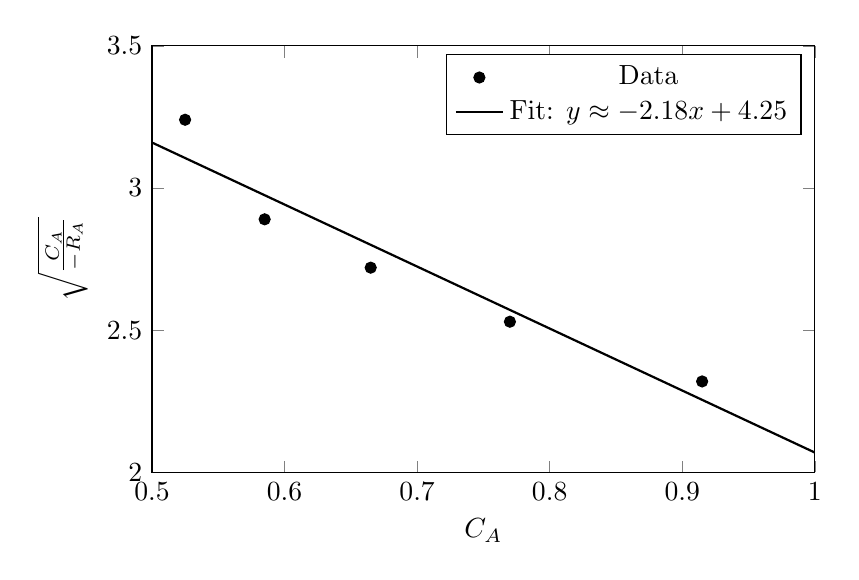
\begin{tikzpicture}
\begin{axis}[
    width=10cm,
    height=7cm,
    xlabel={$ C_A $},
    ylabel={$ \sqrt{\frac{C_A}{-R_A}} $},
    xmin=0.5, xmax=1,
    ymin=2, ymax=3.5
]

% Datapunten
\addplot[
    only marks,
    mark=*,
] coordinates {
    (0.915, 2.32)
    (0.77, 2.53)
    (0.665, 2.72)
    (0.585, 2.89)
    (0.525, 3.24)
};

% Lineaire fit (benaderd)
\addplot[
    domain=0.5:1.0,
    samples=100,
    thick
] {-2.18*x + 4.25};

\legend{Data, Fit: $y \approx -2.18x + 4.25$}

\end{axis}
\end{tikzpicture}
\end{figure}
\fi
Hiermee kunnen we $k_1$ en $k_2$ bepalen.
\[k_1 = \answer{0.055}\]
\[k_2 = \answer{-0.513}\]
\begin{feedback} .
\newline
    Het intercept van de rechte: $\frac{1}{\sqrt{k_1}} = 4.25$.
    \[k_1 = 0.055\]
    De helling van de rechte: $\frac{k_2}{\sqrt{k_1}} = -2.18$. \\
    \[k_2 = -0.51\]
\end{feedback}
\end{question}

\end{document}